\documentclass[convert={outext=.tex.png}]{standalone}
\usepackage{ulem,tikz,xcolor}
\usetikzlibrary{arrows,arrows.meta,calc,fit,positioning,shapes.geometric}

\tikzset{
  pics/database/.style={code={
    \coordinate (-top) at (0,0.5);
    \coordinate (-top-center) at (0,0);
    \coordinate (-bottom) at (0,-2.5);
    \node at (0, 0) {#1};
    \draw (0,0) ellipse (1 and 0.5);
    \draw (-1,0) -- (-1,-2);
    \draw (-1,-2) arc (180:360:1 and 0.5);
    \draw (1,-2) -- (1, 0);
    \fill [gray,opacity=0.5] (-1,0) -- (-1,-2) arc (180:360:1 and 0.5) -- (1,0) arc (0:180:1 and -0.5);
  }}
}

\begin{document}
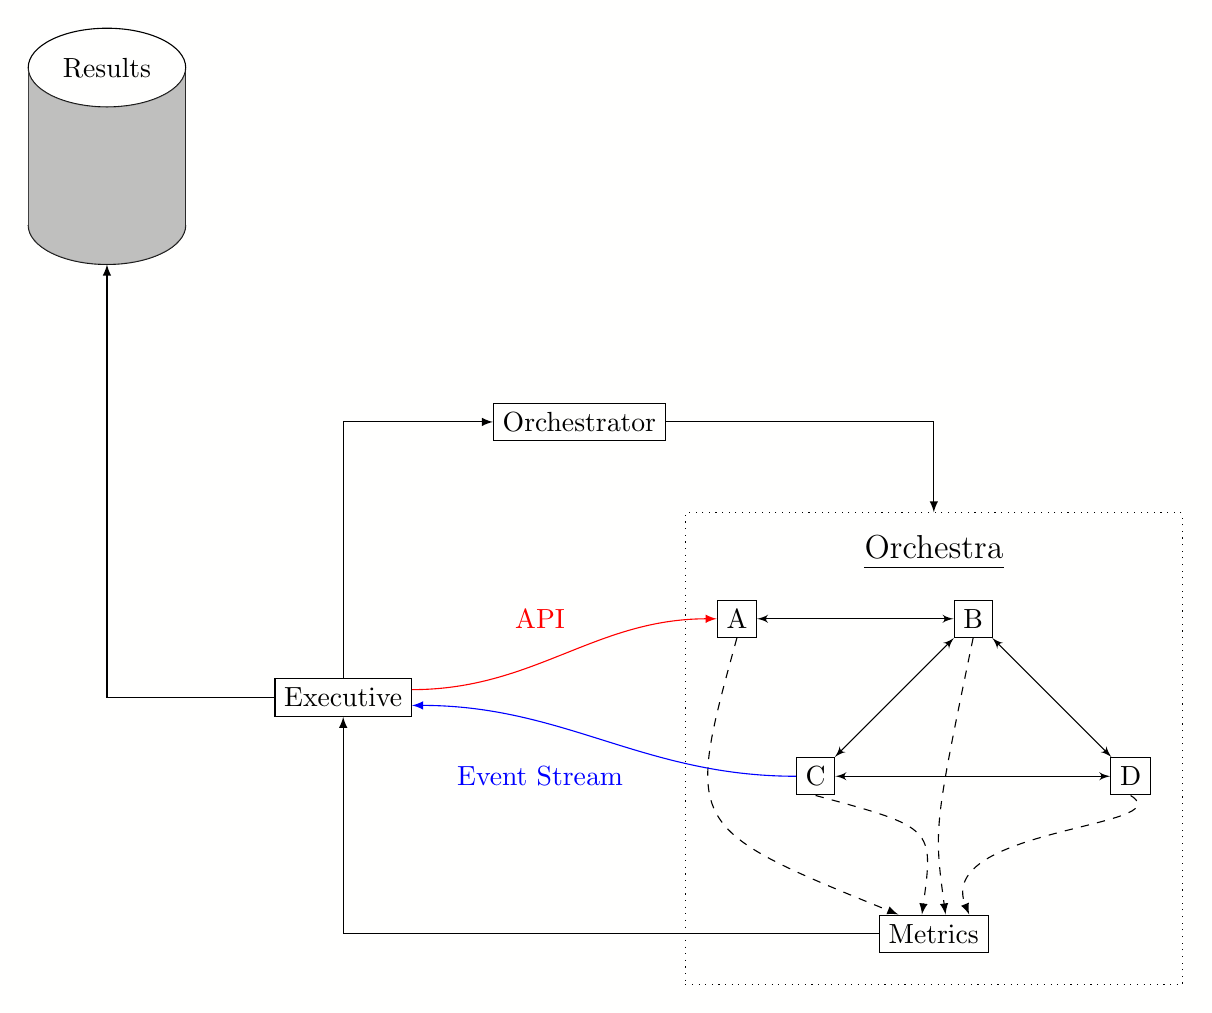
\begin{tikzpicture}
  \pagecolor[RGB]{255,255,254}

  \node[draw] (executive) at (0,-1) {Executive};
  \pic[draw] (results-db) at (-3,7) {database={Results}};
  \node[draw] (orchestrator) at (3,2.5) {Orchestrator};
  \foreach \name/\x/\y in {A/0/0,B/3/0,C/1/2,D/5/2} {
    \node[draw] at ($(5,0)+(\x,-\y)$) (node-\name) {\name};
  }
  \node[draw] (metrics) at (7.5,-4) {Metrics};
  \node[draw,dotted,inner sep=0.4cm,fit={(node-A) (node-B) (node-C) (node-D) (metrics) ($(node-A.north)+(0,0.7)$)}] (orchestra) {};
  \node (orchestra-label) at ($(orchestra.north)-(0,0.5)$) {\large\uline{Orchestra}};
  %\node[draw,below=1cm of orchestra] (metrics) {Metrics};

  \draw[-latex] (executive) |- (orchestrator);
  \draw[-latex] (orchestrator) -| (orchestra.north);
  \draw[-latex] (metrics) -| (executive);
  \draw[-latex] (executive.west) -| (results-db-bottom);

  \draw[latex'-latex'] (node-A) -- (node-B);
  \draw[latex'-latex'] (node-B) -- (node-C);
  \draw[latex'-latex'] (node-C) -- (node-D);
  \draw[latex'-latex'] (node-D) -- (node-B);

  \draw[-latex,dashed]
    (node-A.south)
    .. controls ($(orchestra.south west)+(0,2)$)
       and ($(orchestra.south west)+(0,2)$)
    .. ($(metrics.north)-(0.45,0)$);
  \draw[-latex,dashed]
    (node-B.south)
    .. controls ($(orchestra.south)+(0,2)$)
       and ($(orchestra.south)+(0,2)$)
    .. ($(metrics.north)+(0.15,0)$);
  \draw[-latex,dashed]
    (node-C.south)
    .. controls ($(orchestra.south)+(0,2)$)
       and ($(orchestra.south)+(0,2)$)
    .. ($(metrics.north)-(0.15,0)$);
  \draw[-latex,dashed]
    (node-D.south)
    .. controls ($(orchestra.south east)+(0,2)$)
       and ($(orchestra.south)+(0,2)$)
    .. ($(metrics.north)+(0.45,0)$);

  \draw[-latex,color=red]
    ($(executive.east)+(0,0.1)$)
    to[out=0,in=180,looseness=1]
    (node-A)
    node[at start,xshift=2.5cm] {API};
  \draw[-latex,color=blue]
    (node-C)
    to[out=180,in=0,looseness=1]
    ($(executive.east)-(0,0.1)$)
    node[at start,xshift=2.5cm,yshift=-2cm] {Event Stream};
\end{tikzpicture}
\end{document}
